\documentclass[hyperref,german,beleg,noproblem,notoc,plainarticle]{cgvpub}

\makeatletter
\def\BState{\State\hskip-\ALG@thistlm}
\makeatother
\DeclareMathOperator*{\argmax}{arg\,max}  % in your preamble
\DeclareMathOperator*{\argmin}{arg\,min}  % in your preamble 


%weitere Optionen zum Erg�nzen (in eckigen Klammern):
%
% female	weibliche Titelbezeichnung bei Diplom
% bibnum	numerische Literaturschl�ssel
% final 	f�r Abgabe	
% lof			Abbildungsverzeichis
% lot			Tabellenverzeichnis
% noproblem	keine Aufgabenstellung
% notoc			kein Inhaltsverzeichnis
% twoside		zweiseitig
\author{\textbf{Gruppe 11}\\ Cao,Bozhi\hspace{1em}Gao,Yue\hspace{1em}Jia,Xuehua\hspace{1em}Zhu,Jinyao }
\title{PRAKTIKUMSAUFGABE I}
%\bibfiles{literatur}
%\problem{Text der Aufgabenstellung...}
%\copyrighterklaerung{Hier soll jeder Autor die von ihm eingeholten
%Zustimmungen der Copyright-Besitzer angeben bzw. die in Web Press
%Rooms angegebenen generellen Konditionen seiner Text- und
%Bild"ubernahmen zitieren.}
%\acknowledgments{Die Danksagung..}

\renewcommand\thesection{\arabic{section}.}
\renewcommand\thesubsection{\thesection\arabic{subsection}}
\renewcommand\thefigure{\arabic{figure}}  


\begin{document}
	  
\section{Aufgabe}
\subsection{Analytische L"osung($u_1=5,T_m=10\mathrm{s},t_{step}=1\mathrm{s}$):}
$$ y(t) = u_1\left( 1-e^{-\frac{1}{T_m}(t-t_{step})}\right)=5\left( 1-e^{-\frac{1}{10}(t-1)} \right)   $$
\subsection{Simulationsergebnisse:}
\textbf{VPG ohne Schrittweitensteuerung($t_{step}=1\mathrm{s},u_1=5,h=0.1\mathrm{s}$):}\\
\begin{figure}[htb]
	\centering
	$
	\begin{array}{cc}
	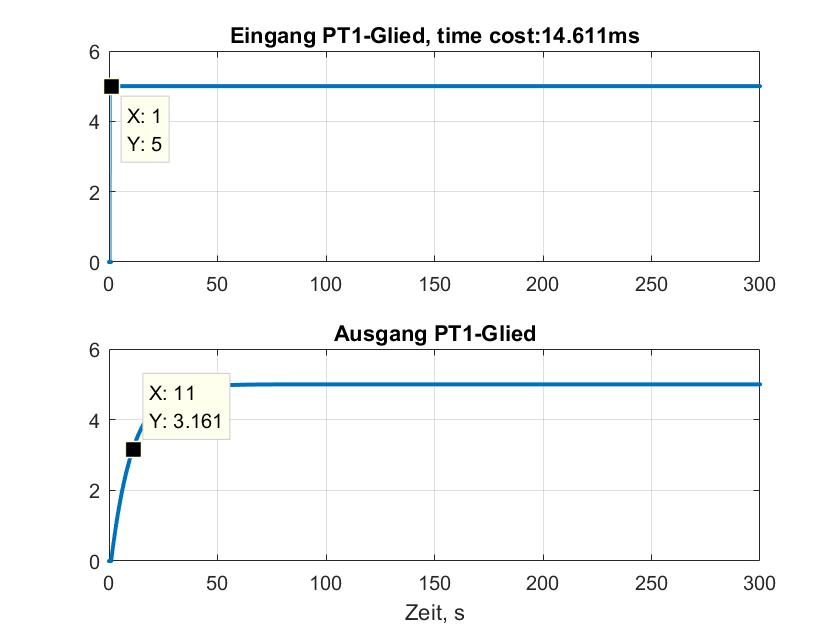
\includegraphics[width=0.45\linewidth]{picture/a1_1} &
	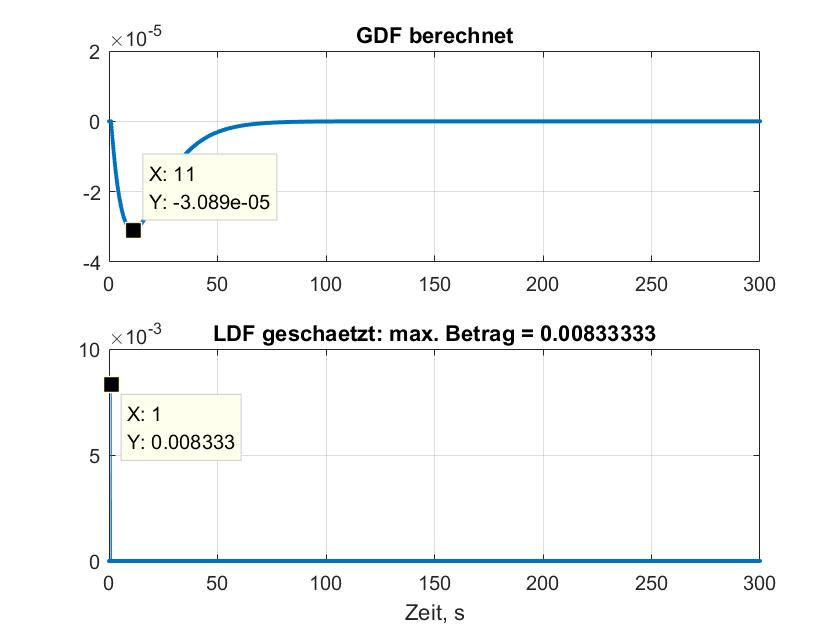
\includegraphics[width=0.45\linewidth]{picture/a1_2}\\
	\text{(a)} & \text{(b)}
	\end{array}
	$
	\caption{(a) F"uhrungsverhalten; (b) Verhalten der Global-/Lokaldiskretisierungsfehler;}
	\label{fig1}
\end{figure}

\subsection{Verifizierung}
Aus der Simulationsergebnisse kann die Zeitkonstante der $\mathrm{PT}_1$ Glied $(11-1=10\mathrm{s})$ abgelesen werden, welche der $T_m$ entsprecht.\\
\textbf{Verhalten der G/LDF an der Sprungstelle($t=1\mathrm{s}$):} die lokale Diskretisierungsfehler "andern sich sprungartig. Der LDF an der Sprungstelle ist deutlich gr"o"ser als an der Ruhelager des Systems. Die GDF erreichen ihre Maxima zum Zeitpunkt $t\approx11\mathrm{s}$.

\newpage
\section{Aufgabe}
\subsection{Bestimmung des Intervalls der Schrittweite:}
\textbf{Maximale Schrittweite $h_{max}$:}\\
Charakteristische Gleichung von $G_1(s)$:\\
$$T_m\lambda+1=0,\text{ mit }T_m=10\mathrm{s}$$
$$\lambda = -\frac{1}{T_m} = -0.1\mathrm{s}^{-1}$$
Nach der Stabilit"atsgebiete f"ur Verbesserte Polygonzugmethode: 
$$\mu=h\cdot\lambda, \text{ mit } |\mu|_{max}=2.0$$
$$\Rightarrow  h_{max} = \frac{|\mu|_{max}}{|\lambda|}=20\mathrm{s}$$

\textbf{Minimale Schrittweite $h_{min}$:}\\
gesch"atzte LDF $\hat{d}$ an der Sprungstelle:\\
wenn $t_{i}+\frac{h}{2}<t_{step}<t_i+h$:\\
$$
\left. 
\begin{array}{l}
k_1 =0  \\
k_2 =0  \\
k_3 = \frac{u_1}{T_m} 
\end{array}
\right\rbrace \Rightarrow \hat{d_1} = \frac{h}{6}\cdot k_3=\frac{h}{6}\cdot\frac{u_1}{T_m} 
$$

wenn $t_i<t_{step}<t_{i}+\frac{h}{2}$:\\
$$
\left.
\begin{array}{l}
k_1 =0  \\
k_2 =\frac{u_1}{T_m}\\
k_3 = \frac{u_1}{T_m}\cdot\left( 1-\frac{2h}{T_m} \right)
\end{array}
\right\rbrace \Rightarrow \hat{d_2} = \frac{h}{6}\cdot\left( -2k_2+k_3 \right) = -\frac{h}{6}\cdot\frac{u_1}{T_m}\cdot\left( 1+\frac{2h}{T_m} \right) 
$$
Anforderung($\frac{2h}{T_m}\ll1$):
$$ |\hat{d_1}|=\left| \frac{h}{6}\cdot\frac{u_1}{T_m}\right|  \approx|\hat{d_2}|\leq\varepsilon_{LDF} $$
mit $u_1=5,T_m=10\mathrm{s},\varepsilon_{LDF}=10^{-6}$
$$ \Rightarrow h_{min} \leq \frac{6}{\left| \frac{u_1}{T_m} \right|}\cdot\varepsilon_{LDF}=1.2\times10^{-5}\mathrm{s}$$

\newpage
\subsection{Simulationsergebnisse:}
\textbf{VPG mit Schrittweitensteuerung($t_{step}=1\mathrm{s},u_2=5,h_{init}=0.5\mathrm{s},\varepsilon_{LDF}=10^{-6}$):}\\
\begin{figure}[htb]
	\centering
	$
	\begin{array}{cc}
	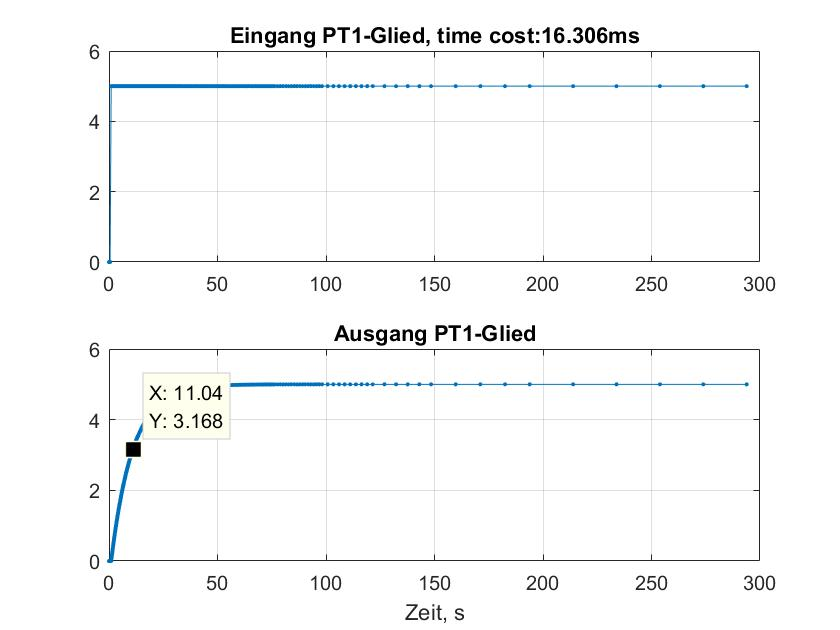
\includegraphics[width=0.45\linewidth]{picture/a2_1} &
	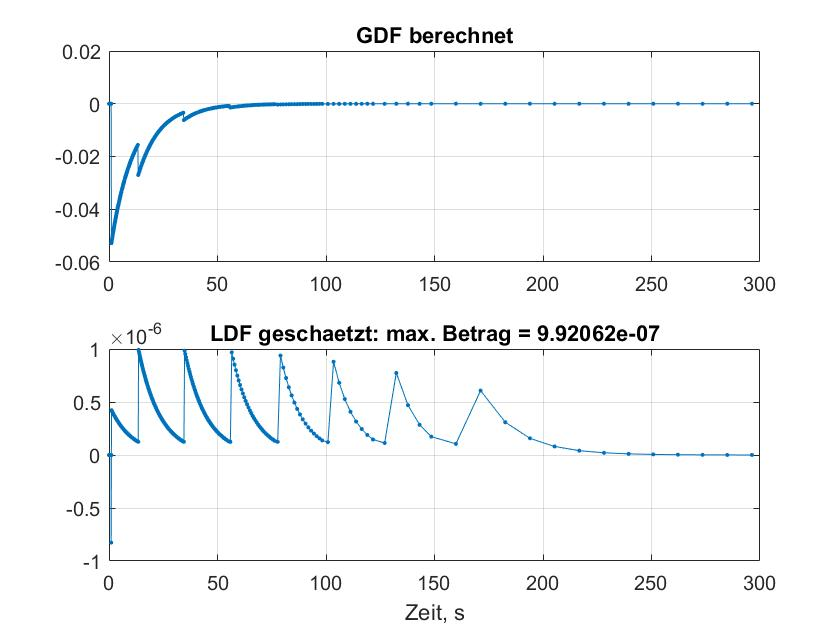
\includegraphics[width=0.45\linewidth]{picture/a2_2}\\
	\text{(a)} & \text{(b)}\\
	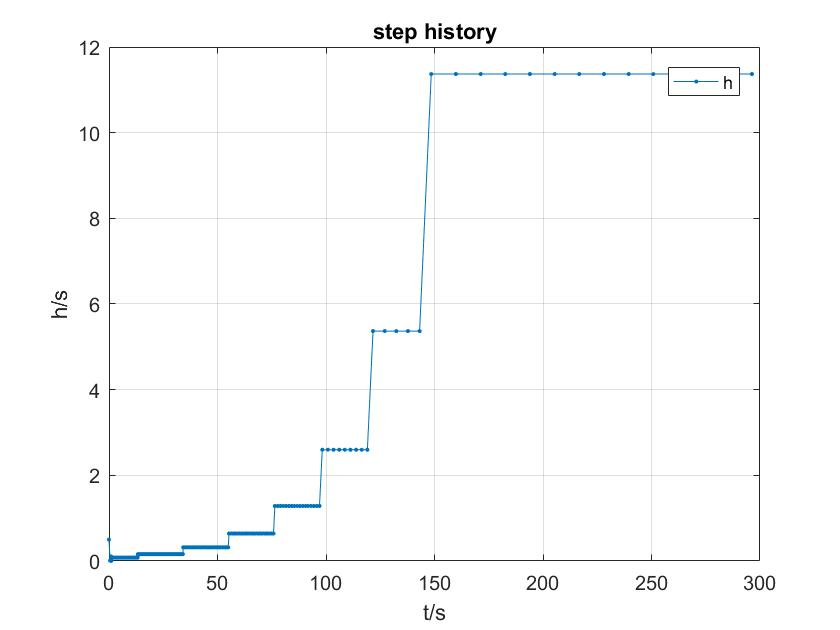
\includegraphics[width=0.45\linewidth]{picture/a2_3} &
	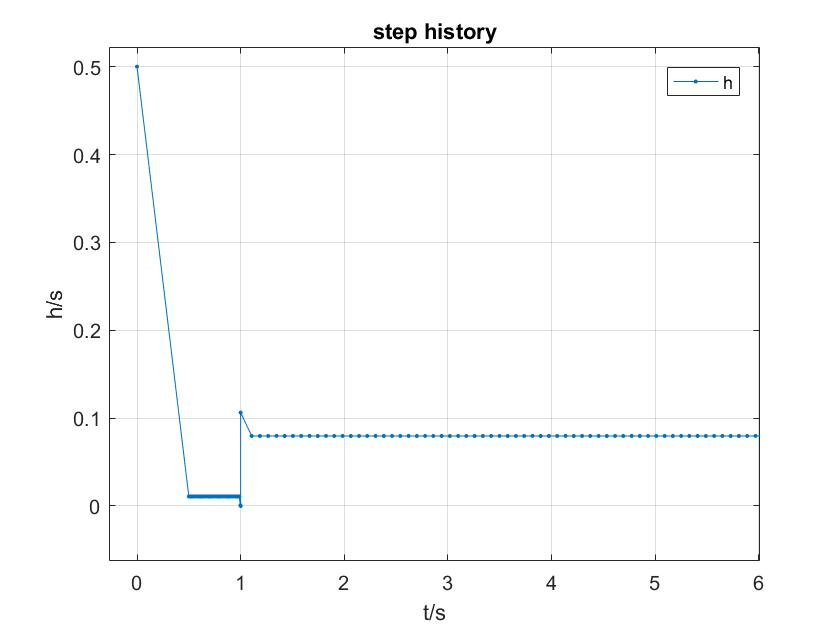
\includegraphics[width=0.45\linewidth]{picture/a2_4}\\
	\text{(c)} & \text{(d)}
	\end{array}
	$
	\caption{(a) F"uhrungsverhalten; (b) Verhalten der Global-/Lokaldiskretisierungsfehler; (c) Verlauf der Schrittweite; (d) Verlauf der Schrittweite in der N"ahe der Sprungstelle;}
	\label{fig2}
\end{figure}

\subsection{Verifizierung}
Aus der Simulationsergebnisse kann die Zeitkonstante der $\mathrm{PT}_1$ Glied $(\approx10\mathrm{s})$ abgelesen werden, welche der $T_m$ entsprecht.\\
\textbf{Verhalten der Schrittweite in der N"ahe der Sprungstelle($t=1\mathrm{s}$):} die Schrittweite "andert sich nahe vor der Sprungstelle sprungartig und deutlich kleiner, nach der Sprungstelle vergr"o"sert sie sich.\\
\textbf{Verlauf der LDF:} die LDF sind in der Simulation immer auf $\varepsilon_{LDF}=10^{-6}$ begrenzt.

\newpage
\section{Aufgabe}
\subsection{Simulationsergebnisse:}
\textbf{VPG mit Schrittweitensteuerung($t_{step}=1\mathrm{s},u_2=0.17,h_{init}=0.001\mathrm{s},\varepsilon_{LDF}=10^{-10}$):}\\
\begin{figure}[htb]
	\centering
	$
	\begin{array}{cc}
	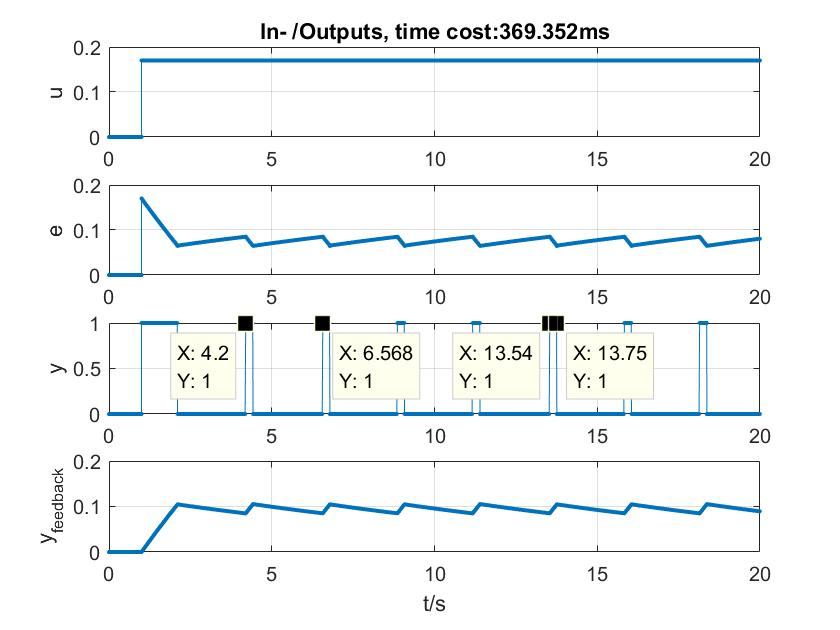
\includegraphics[width=0.45\linewidth]{picture/a3_1} &
	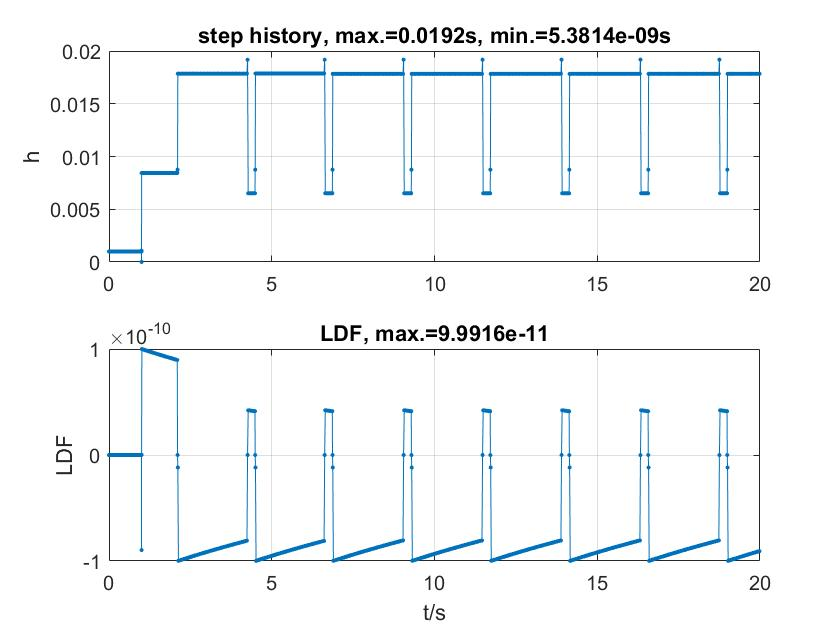
\includegraphics[width=0.45\linewidth]{picture/a3_2}\\
	\text{(a)} & \text{(b)}
	\end{array}
	$
	\caption{(a) Eingang und alle Blockausg"ange; (b) Verlauf der Schrittweite und LDF;}
	\label{fig3}
\end{figure}

\textbf{VPG ohne Schrittweitensteuerung($t_{step}=1\mathrm{s},u_2=0.17,h=0.001\mathrm{s}$):}\\
\begin{figure}[htb]
	\centering
	$
	\begin{array}{cc}
	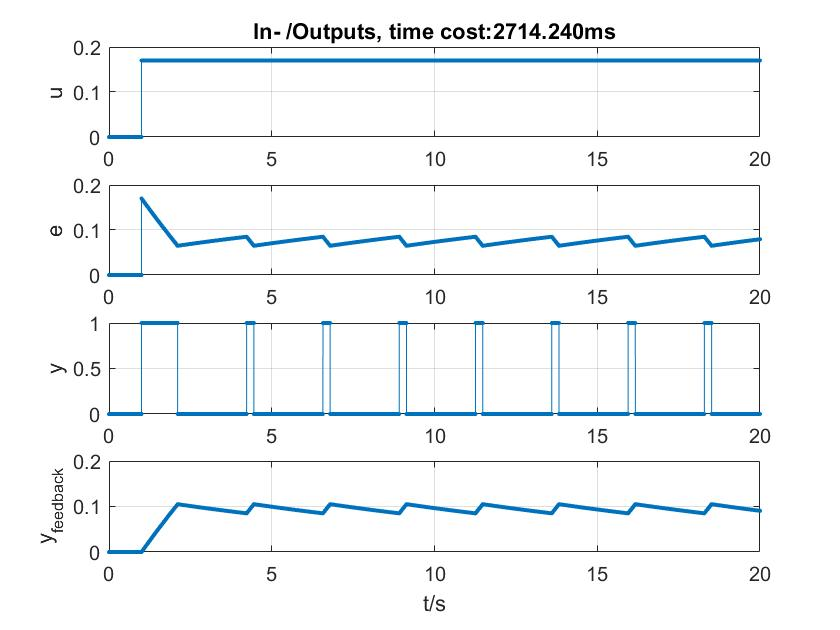
\includegraphics[width=0.45\linewidth]{picture/a3_3} &
	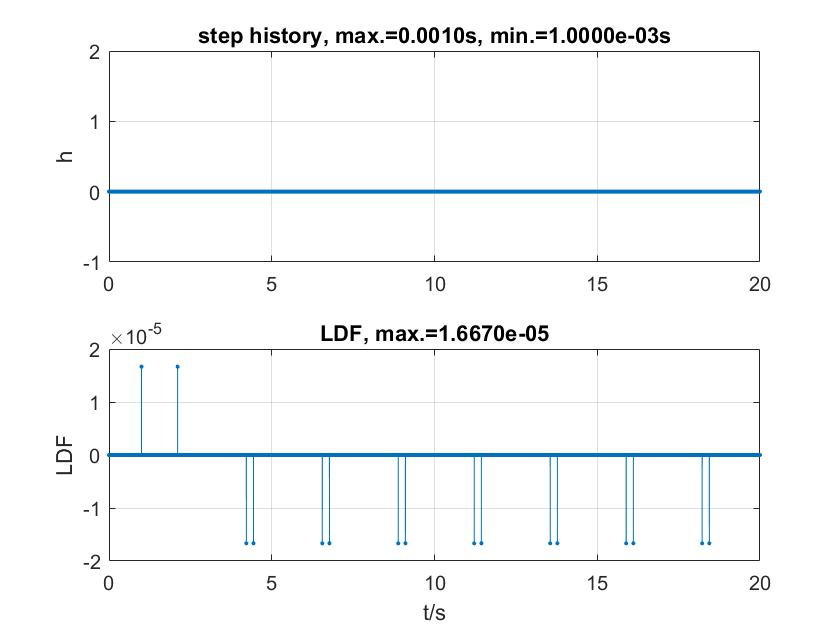
\includegraphics[width=0.45\linewidth]{picture/a3_4}\\
	\text{(a)} & \text{(b)}
	\end{array}
	$
	\caption{(a) Eingang und alle Blockausg"ange; (b) Verlauf der Schrittweite und LDF;}
	\label{fig4}
\end{figure}
\subsection{Verifizierung}
Aus der Gleichung:
$$\tau_e=-T_m\cdot\ln\left( 1-\frac{h_e-h_a}{1+h_e-|u_2|}\right) $$
$$\tau_p=T_m\cdot\left[ \ln\frac{1-h_a/|u_2|}{1-h_e/|u_2|}-\ln\left(1-\frac{h_e-h_a}{1+h_e-|u_2|}\right)\right] $$
mit 
$$u_e=0.17,h_a=0.065,h_e=0.085,T_m=10\mathrm{s}$$\\
erh�lt man:
$$ \tau_e=0.2210\mathrm{s},\hspace{1em}\tau_p=2.3341\mathrm{s} $$
Aus Simulation(Abbildung \ref{fig3}):
$$ \hat{\tau}_e=0.21\mathrm{s},\hspace{1em}\hat{\tau}_p=2.368\mathrm{s} $$
die Simulationsergebnisse den analytischen Werten entsprechen.

\textbf{Vergleichen(mit/ohne Schrittweitensteurung des VPG-Algorithmus):}\\
um eine "ahnliche Genauigkeit(LDF Toleranz) zu erreichen, braucht das VPG-Algorithmus ohne Schritt-weitensteurung deutlich mehr Rechenzeit als das mit Schrittweitensteurung.

\subsection{Weitere Experimente mit $u_{22}=-0.25,u_{23}=0.49$:}
\begin{figure}[htb]
	\centering
	$
	\begin{array}{cc}
	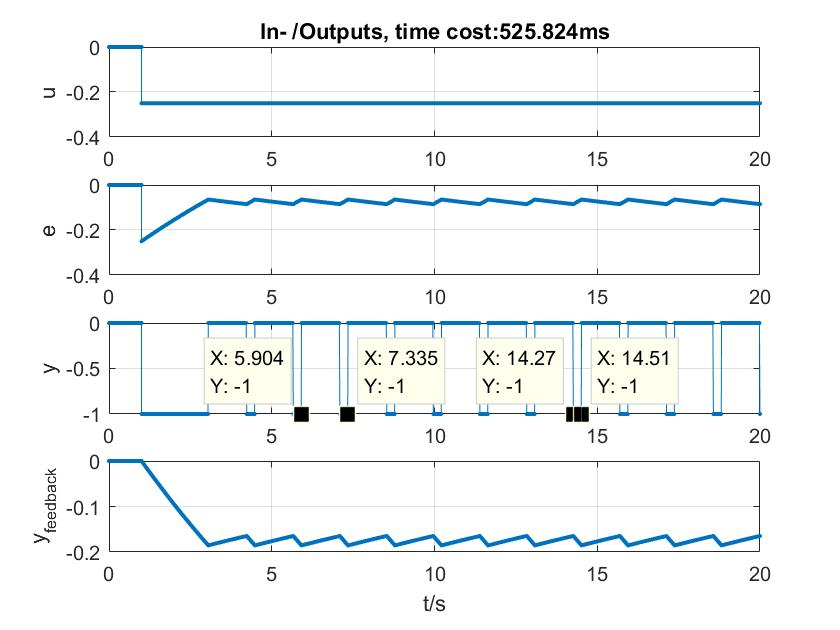
\includegraphics[width=0.45\linewidth]{picture/a3_5} &
	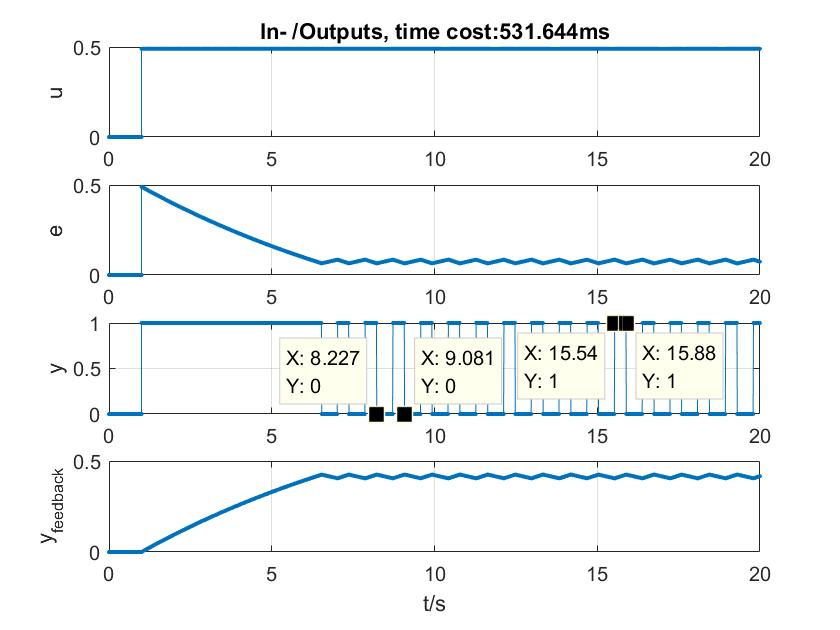
\includegraphics[width=0.45\linewidth]{picture/a3_6}\\
	\text{(a)} & \text{(b)}
	\end{array}
	$
	\caption{(a) $u_2=u_{22}=-0.25$; (b) $u_2=u_{23}=0.49$;}
	\label{fig5}
\end{figure}
\centering
\begin{tabular}{l||c|c|c|c}
	\hline 
	& $\tau_e(\mathrm{s})$ & $\hat{\tau}_e(\mathrm{s})$ & $\tau_p(\mathrm{s})$ & $\hat{\tau}_p(\mathrm{s})$ \\ 
	\hline 
	$u_2 = -0.25$& 0.2424 & 0.24 & 1.3865 & 1.431 \\ 
	\hline 
	$u_2 = \hspace{0.72em}0.49$& 0.3419 & 0.34 & 0.8239 & 0.854 \\ 
	\hline 
\end{tabular} 

\end{document} 